%
\documentclass[12pt, oneside]{article}
\usepackage[margin=0.85in]{geometry}
\linespread{1}
\usepackage{xcolor}
\usepackage[colorlinks=false, linkbordercolor=white, citebordercolor=white, 
    filebordercolor=white, urlbordercolor=white]{hyperref}
    
\usepackage{graphicx}
\usepackage[utf8]{inputenc}
\usepackage[T1]{fontenc}
\usepackage{minted}

\usepackage{fancyhdr}
\pagestyle{fancy}
\renewcommand{\headrulewidth}{0.4pt}
\fancyhead{}
\fancyhead[L]{CS6700 Reinforcement Learning} 
\fancyhead[R]{Varun EE16B068} 
\fancyfoot{}
\fancyfoot[C]{\thepage}

\usepackage{titlesec}
\titlespacing{\chapter}{0pt}{*4}{*2.5}

\titleformat{\chapter}{\normalfont\huge\bf}{\thechapter}{20pt}{\huge\bf}



\usepackage{listings}
\definecolor{dgray}{gray}{0.35} 
\definecolor{lgray}{gray}{0.95} 

\lstset{ 
language=Python, 
basicstyle=\ttfamily\small, 
backgroundcolor=\color{lgray},
commentstyle=\ttfamily\small\itshape\color{dgray}, 
showstringspaces=false, 
numbers=left, 
numberstyle=\ttfamily\small, 
stepnumber=1, 
firstnumber=last, 
breaklines=T} 

\begin{document}

\begin{titlepage}
    \begin{center}
        \vspace*{1cm}
        
        \Huge
          \textbf{Reinforcement Learning CS6700}
        
        \vspace{0.5cm}
        \LARGE
        Fall 2018
        
        \vspace{1.5cm}
        
        \textbf{Assignment 4}
   		  \vspace{1.5cm}
        
        \textbf{Report}
       
        \vfill
        
        Author: Varun Sundar
        
        \vspace{0.8cm}
          \Large
        EE16B068 \\
        \vspace{0.5cm}
       18th October 2018
        
    \end{center}
\end{titlepage}
\addtocontents{toc}{~\hfill\textbf{Page}\par}
\section {Implementation and Technical Notes}

The code uses python 3.6 with sub-modules for questions. The repository adheres to the following:
\begin{itemize}
\item \textit{Numpy style} documentation for the module and exposed functions. 
\item A \textit{requirements.txt }for pip installing packages.
\item  Reproducible logs and reports.
\end{itemize}

\section{Question 1: Grid World Problem}

We reuse the module \textit{bellman.py} written for \textit{Assignment 2}.

Modelling the grid-world:
\begin{itemize}
\item We use a 2D array, referenced by flattened indices for operating upon.
\item Indices go from $(0,0)$ to $(9,9)$. 
\item Again, $P$, $r$, and $J$ are modelled by tensors.
\item \textit{Wormholes}: Correspond to probabilities of 1 towards transition.
\item \textit{Terminal}: Collect a one time, at transit reward of $+100$. 
\end{itemize}

\subsection{Code Blocks (pertinent only)}

\begin{lstlisting}
P=np.zeros((100,100,4))

# Up is +10; 0
    if (i < 90):
        P[i, i + 10, 0] = 0.8
    else:
        P[i, i, 0] = 0.8

    if i % 10 < 9:
        P[i, i + 1, 0] = 0.2 / 3
    else:
        P[i, i, 0] = 0.2 / 3
    if i % 10 > 0:
        P[i, i - 1, 0] = 0.2 / 3
    else:
        P[i, i, 0] = 0.2 / 3

    if (i > 9):
        P[i, i - 10, 0] = 0.2 / 3
    else:
        P[i, i, 0] = 0.2 / 3
        
    # Down is -10 ...
    # Left is -1 ....
    # Right is +1 ...
    
# Wormholes, multiple outputs
for i in [32, 42, 52, 62]:
    for j in range(4):
        P[0, i, j] = 0.25
        P[0, 1, j] = 0
        P[0, 0, j] = 0
        P[0, 10, j] = 0
        
        ....
# Terminal stage

P[terminal,terminal,:]=1
if (terminal%10)<9:
    P[terminal,terminal+1,:]=0
if (terminal%10)>0:
    P[terminal,terminal-1,:]=0
if (terminal<90):
    P[terminal,terminal+10,:]=0
if (terminal>9):
    P[terminal,terminal-10,:]=0

r=np.zeros((100,100,4))
r[:,terminal,:]=100
# Collect reward only once
r[terminal,terminal,:]=0
\end{lstlisting}

\subsection{Part 2}

We stop when the maximal absolute difference (np.max(np.abs()) of $J_i$ and $J_{i+1}$ falls below a certain $\epsilon$. For the sake of these three questions, we use $\epsilon = 1e-4$. \\

Nonetheless, for value iteration, all plots include upto 20 stages for clarity.

The intuition for this follows from the fact that $T$ is a contraction mapping, hence its repeated operations produce a Cauchy sequence in metric complete space. We have used to strength this fact.

\subsubsection{Part 2-a}

We plot the convergence of $J$ (as $max_s | J_{i+1}(s) - J_s(i) | $ ) and the change in actions (as $\sum_s \pi_{i+1}(s) \neq \pi_i(s)$ ).

We notice that it takes around 12 - 15 iterations for value iteration to converge, while only 3-4 for policy iteration. Here, convergence implies that the differences in $J$ and $\pi$ as measured above tend to zero. This shows the superior convergence of policy iteration in comparison to value iteration.

\begin{figure}[h]
\begin{subfigure}
\centering
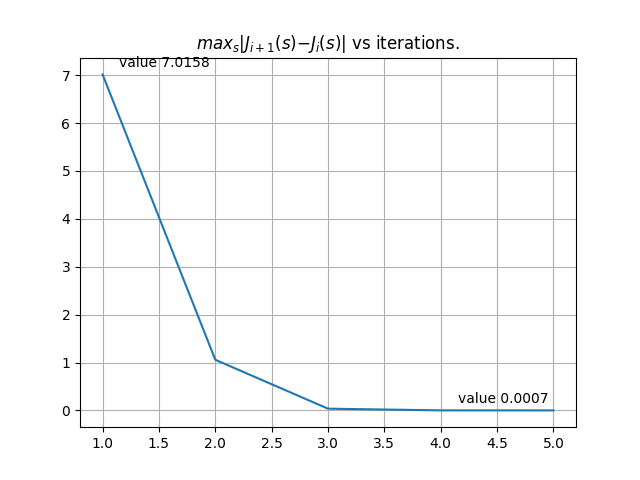
\includegraphics[angle=0,width=0.6\textwidth]{hw4/logs/policy_iter_t=99_N=20/convergence-difference-till-6.png}
\caption{ \textbf{Policy Iteration}Convergence of $J_i$ for \textbf{Terminal State (9,9)}}
\end{subfigure}

\begin{subfigure}
\centering
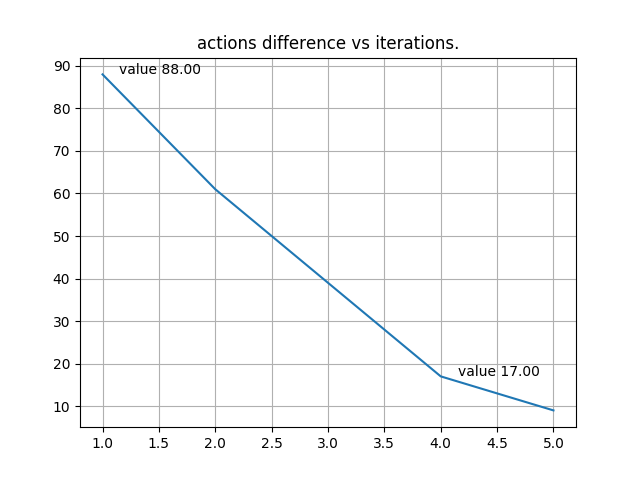
\includegraphics[angle=0,width=0.6\textwidth]{hw4/logs/policy_iter_t=99_N=20/actions-difference-till-6.png}
\caption{ \textbf{Policy Iteration}Convergence of $\pi_i$ for \textbf{Terminal State (9,9)}}
\end{subfigure}
\end{figure}

\begin{figure}[h]
\begin{subfigure}
\centering
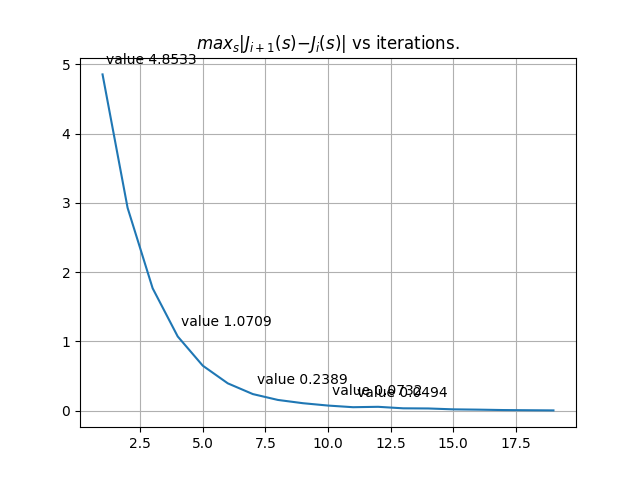
\includegraphics[angle=0,width=0.6\textwidth]{hw4/logs/value_iter_t=99_N=20/convergence-difference-till-20.png}
\caption{ \textbf{Value Iteration}Convergence of $J_i$ for \textbf{Terminal State (9,9)}}
\end{subfigure}

\begin{subfigure}
\centering
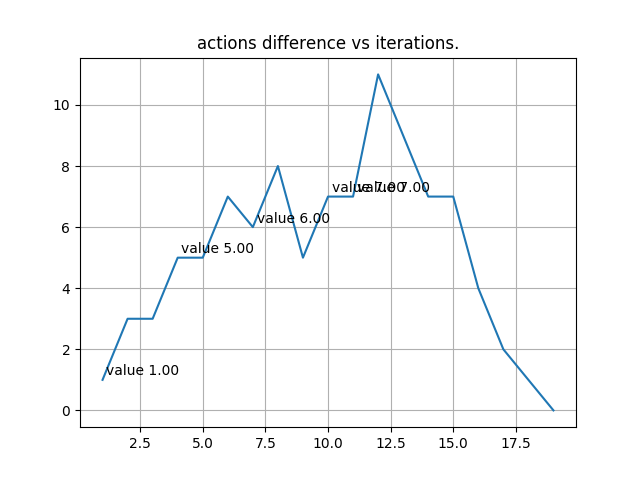
\includegraphics[angle=0,width=0.6\textwidth]{hw4/logs/value_iter_t=99_N=20/actions-difference-till-20.png}
\caption{ \textbf{Value Iteration}Convergence of $\pi_i$ for \textbf{Terminal State (9,9)}}
\end{subfigure}
\end{figure}

\subsubsection{Part 2b}

We now compare the convergence by plotting $J(s)$ for three random states. (We use numpy's randint function to choose the numbers).

Again, we notice faster convergence for policy iteration. The reason policy iteration converges faster is because of the policy evaluation step being done as a matrix inversion step. (A similar analogy to least square fitting with either \textit{Moore Pseudo inverse} versus \textit{gradient descent}). In our case, the number of states is small, and so, this is feasible. In cases where the state space is large, we have to resort to approximate policy evaluation methods.

\begin{figure}[h]
\begin{subfigure}
\centering
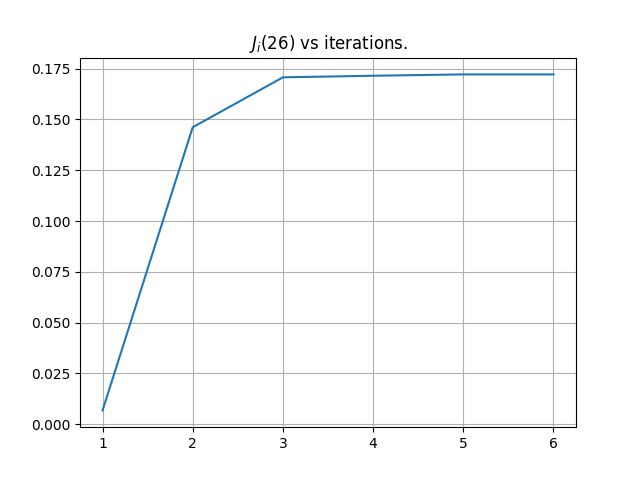
\includegraphics[angle=0,width=0.6\textwidth]{hw4/logs/policy_iter_t=99_N=20/convergence-till-6-state-26.png}
\caption{ \textbf{Policy Iteration}Convergence of $J_i(s)$ with $s =$26 for \textbf{Terminal State (9,9)}}
\end{subfigure}

\begin{subfigure}
\centering
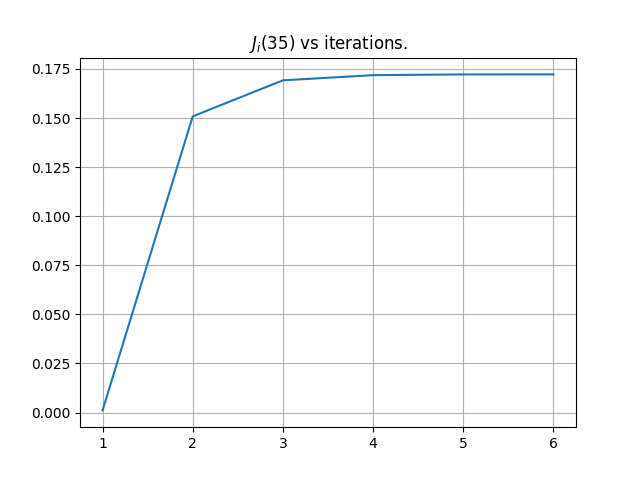
\includegraphics[angle=0,width=0.6\textwidth]{hw4/logs/policy_iter_t=99_N=20/convergence-till-6-state-35.png}
\caption{ \textbf{Policy Iteration}Convergence of $J_i(s)$ with $s =$35 for \textbf{Terminal State (9,9)}}
\end{subfigure}

\begin{subfigure}
\centering
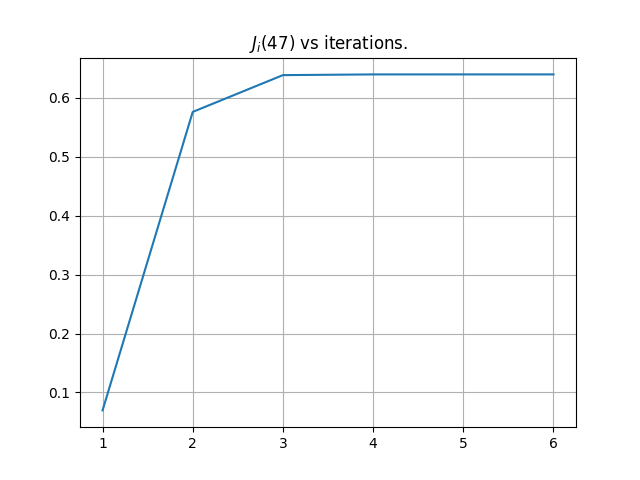
\includegraphics[angle=0,width=0.6\textwidth]{hw4/logs/policy_iter_t=99_N=20/convergence-till-6-state-47.png}
\caption{ \textbf{Policy Iteration}Convergence of $J_i(s)$ with $s =$ 47 for \textbf{Terminal State (9,9)}}
\end{subfigure}
\end{figure}

\begin{figure}[h]
\begin{subfigure}
\centering
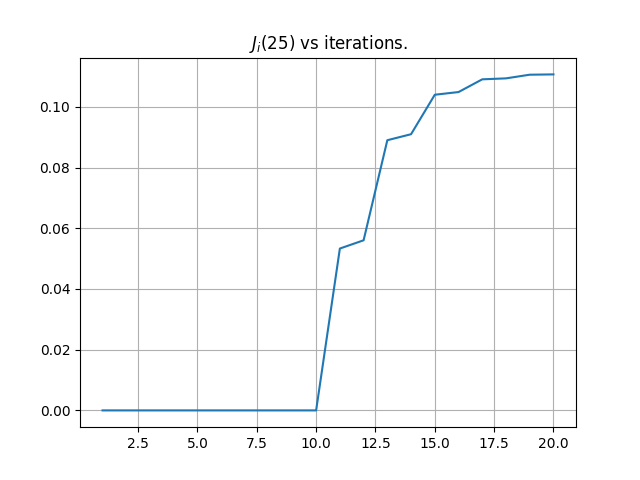
\includegraphics[angle=0,width=0.6\textwidth]{hw4/logs/value_iter_t=99_N=20/convergence-till-20-state-25.png}
\caption{ \textbf{Value Iteration}Convergence of $J_i(s)$ with $s =$25 for \textbf{Terminal State (9,9)}}
\end{subfigure}

\begin{subfigure}
\centering
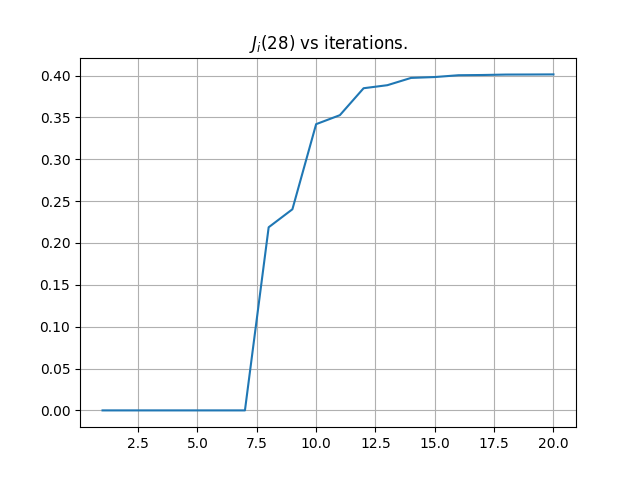
\includegraphics[angle=0,width=0.6\textwidth]{hw4/logs/value_iter_t=99_N=20/convergence-till-20-state-28.png}
\caption{ \textbf{Value Iteration}Convergence of $J_i(s)$ with $s =$28 for \textbf{Terminal State (9,9)}}
\end{subfigure}

\begin{subfigure}
\centering
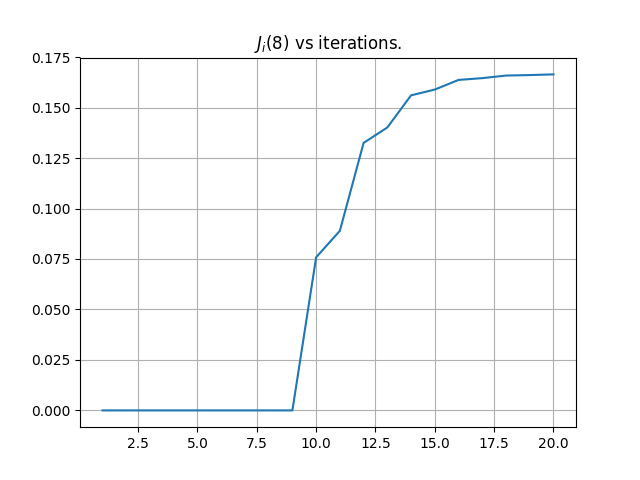
\includegraphics[angle=0,width=0.6\textwidth]{hw4/logs/value_iter_t=99_N=20/convergence-till-20-state-8.png}
\caption{ \textbf{Value Iteration}Convergence of $J_i(s)$ with $s =$ 8 for \textbf{Terminal State (9,9)}}
\end{subfigure}
\end{figure}


\subsection{Part 3,4}

We show the plots of $J$ and \textit{actions} as heatmaps and quiver plots respectively. \\

Plots on pages 12 to 17. \\

Comments on the plots after absolute difference convergence below a pre-determined threshold:
\begin{itemize}
\item  Wormholes are skipped wherever they lead away from the terminal state. (1 in case of (9,9), 2 in case of (3,0)).
\item  Reward to go is minimal at terminal state. (since once acquired, you terminate the game).
\item  The general policy is to either choose an apt wormhole or the direct shortest path to the terminal state.
\item  Since the probability in the intended action (Up when chosen up) is dominant, we see similar actions. If this were not the case, we could see non-obvious actions.
\item Colliding into the walls (and thereby retaining state) is discouraged, unless you happen to be at the terminal state.
\item Thus, this policy is "greedy" and does not take into account any time-variant phenomena, memory etc. Neither does solving this given grid require this.
\end{itemize}

\subsection{Code Snippet for Part 3}

\begin{lstlisting}
def quiver_actions(actions,terminal=args.terminal,stage=0, save_path=None,supress=False):
    '''
    Plot a quiver plot of the policy
    '''
    def _action_u(u):
        '''
        Horz quiver
        -1,1 if u == left or right
        0 else
        '''
        if u==2:
            return -1
        elif u==3:
            return 1
        else:
            return 0
    def _action_v(u):
        '''
        Vert quiver
        -1,1 if u == down or up
        0 else
        '''
        if u==0:
            return 1
        elif u==1:
            return -1
        else:
            return 0
    
    X=Y=np.arange(0.5,10.5,1)
    U= np.array([_action_u(a) for a in actions]).reshape((10,10))
    V= np.array([_action_v(a) for a in actions]).reshape((10,10))
    q=plt.quiver(X,Y,U,V)
    plt.quiverkey(q,X=8, Y=8, U=1,label='Quiver key, length = 1', labelpos='E')
    plt.title(f"Quiver state plot at stage {stage}")

    major_ticks = np.arange(0, 10, 1)

    # Wormholes 1
    for j in range(3,8):
        plt.scatter(2.5,j+0.5,s=225,color=colors['red'])
        plt.text(2.5, j + 0.5, 'IN1')
    # Exit 1
    plt.scatter(0.5,0.5,s=225,color=colors['maroon'])
    plt.text(0.5, 0.5, 'OUT1')

    # Wormholes 2
    plt.scatter(7.5,1.5,s=225,color=colors['grey'])
    plt.text(7.5, 1.5, 'IN2')
    plt.scatter(7.5,9.5,s=225,color=colors['lightgrey'])
    plt.text(7.5, 9.5, 'OUT2')

    # Terminal State
    a=args.terminal//10+0.5
    b=args.terminal%10+0.5
    plt.scatter(b,a,s=256,color=colors['green'])
    plt.text(b,a, 'TERMINAL')

    plt.xlim((0,10))
    plt.ylim((0,10))
    plt.xticks(major_ticks)
    plt.yticks(major_ticks)

    plt.grid(True)

    if save_path:
        plt.savefig(os.path.join(save_path,f"quiver-{stage}.png"))
    if not supress:
        plt.show()
    else:
        plt.close()
\end{lstlisting}





\begin{figure}[h]
\begin{subfigure}
\centering
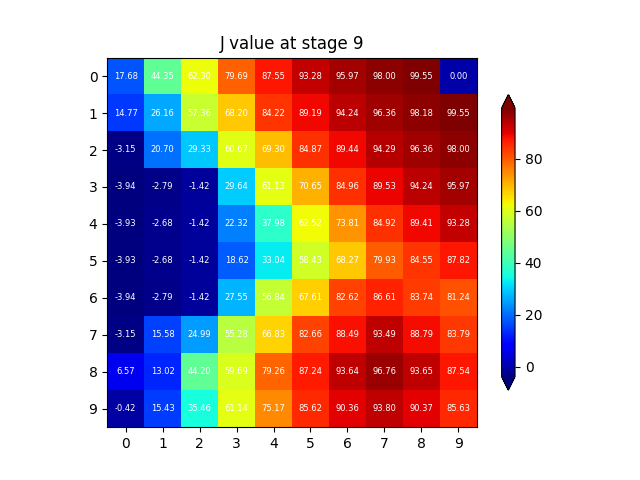
\includegraphics[angle=0,width=0.6\textwidth]{hw2/logs/t=99_N=10/J-heatmap-9.png}
\caption{Heat-map of $J_i$ till $N=10$ for \textbf{Terminal State (9,9)}}
\end{subfigure}

\begin{subfigure}
\centering
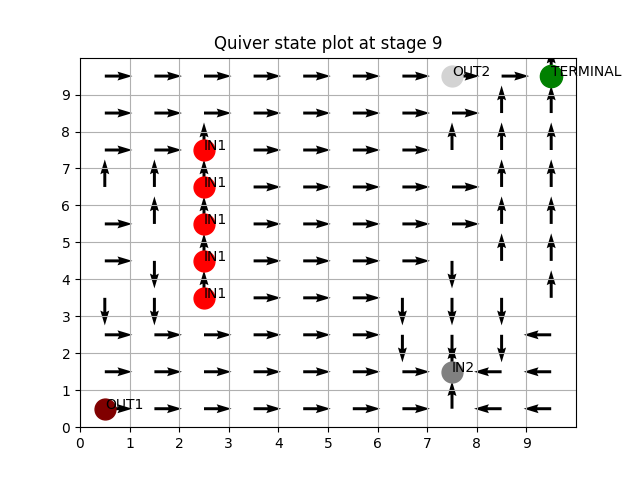
\includegraphics[angle=0,width=0.6\textwidth]{hw2/logs/t=99_N=10/quiver-9.png}
\caption{Quiver plot of $\pi$ till $N=10$ for \textbf{Terminal State (9,9)}}
\end{subfigure}
\end{figure}

\begin{figure}[h]
\begin{subfigure}
\centering
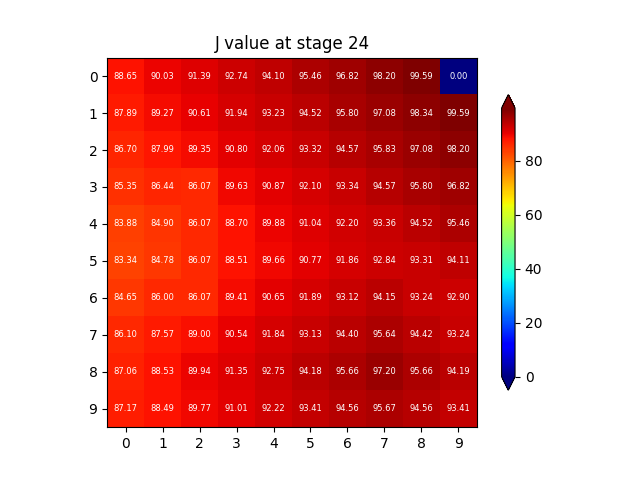
\includegraphics[angle=0,width=0.6\textwidth]{hw2/logs/t=99_N=25/J-heatmap-24.png}
\caption{Heat-map of $J_i$ till $N=25$ for \textbf{Terminal State (9,9)}}
\end{subfigure}

\begin{subfigure}
\centering
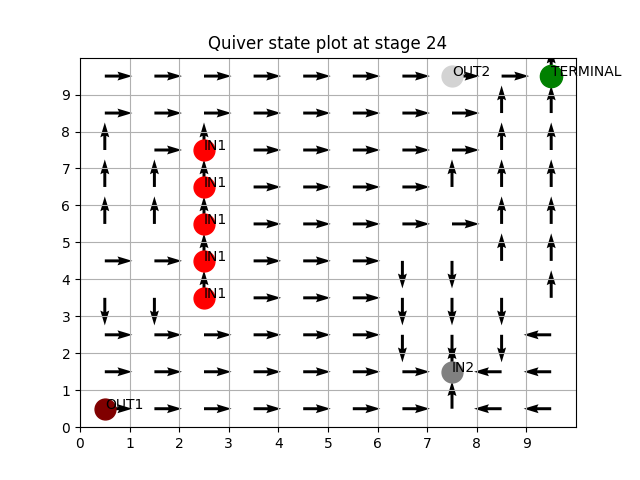
\includegraphics[angle=0,width=0.6\textwidth]{hw2/logs/t=99_N=25/quiver-24.png}
\caption{Quiver plot of $\pi$ till $N=25$ for \textbf{Terminal State (9,9)}}
\end{subfigure}
\end{figure}
\begin{figure}[h]
\begin{subfigure}
\centering
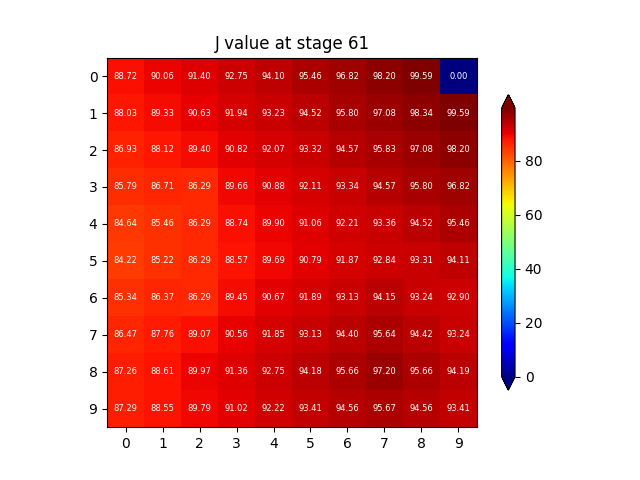
\includegraphics[angle=0,width=0.6\textwidth]{hw2/logs/t=99_N=-1/J-heatmap-61.png}
\caption{Heat-map of $J_i$ till absolute difference convergence for \textbf{Terminal State (9,9)}}
\end{subfigure}

\begin{subfigure}
\centering
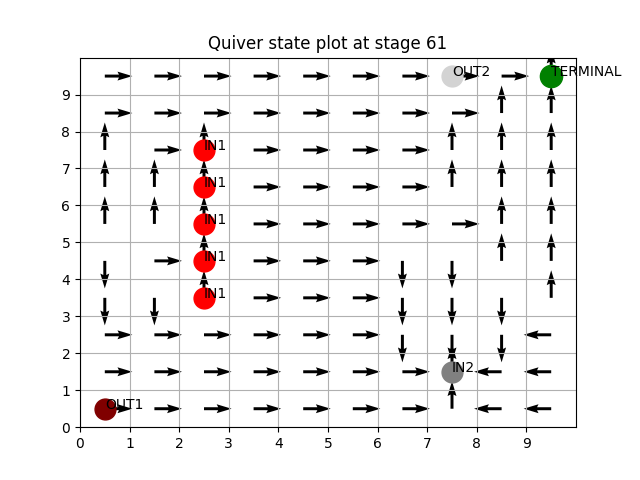
\includegraphics[angle=0,width=0.6\textwidth]{hw2/logs/t=99_N=-1/quiver-61.png}
\caption{Quiver plot of $\pi$  till absolute difference convergence for \textbf{Terminal State (9,9)}}
\end{subfigure}
\end{figure}

\begin{figure}[h]
\begin{subfigure}
\centering
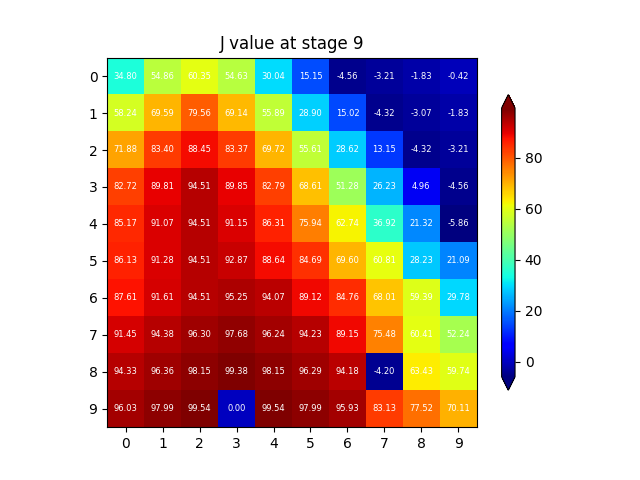
\includegraphics[angle=0,width=0.6\textwidth]{hw2/logs/t=3_N=10/J-heatmap-9.png}
\caption{Heat-map of $J_i$ till $N=10$ for \textbf{Terminal State (3,0)}}
\end{subfigure}

\begin{subfigure}
\centering
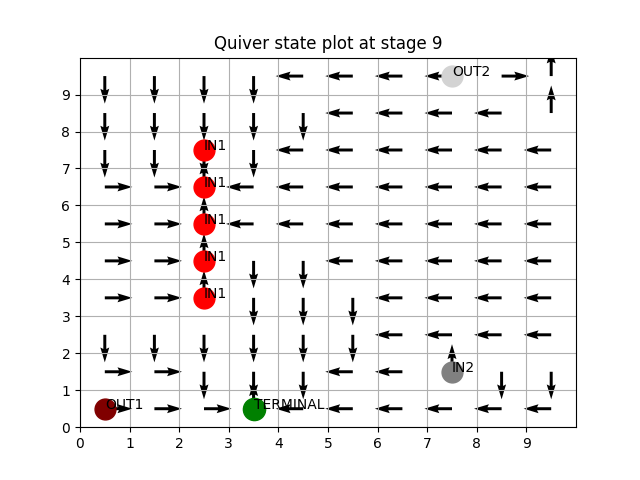
\includegraphics[angle=0,width=0.6\textwidth]{hw2/logs/t=3_N=10/quiver-9.png}
\caption{Quiver plot of $\pi$ till $N=10$ for \textbf{Terminal State (3,0)}}
\end{subfigure}
\end{figure}

\begin{figure}[h]
\begin{subfigure}
\centering
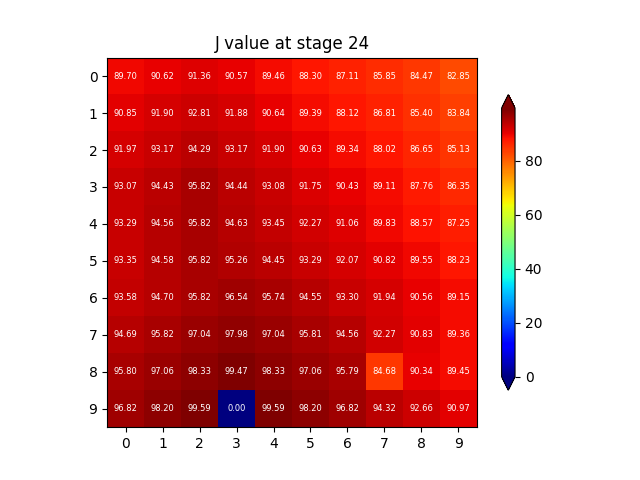
\includegraphics[angle=0,width=0.6\textwidth]{hw2/logs/t=3_N=25/J-heatmap-24.png}
\caption{Heat-map of $J_i$ till $N=25$ for \textbf{Terminal State (3,0)}}
\end{subfigure}

\begin{subfigure}
\centering
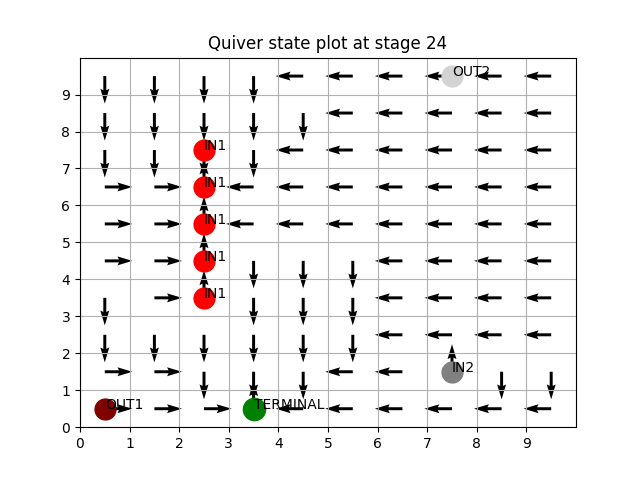
\includegraphics[angle=0,width=0.6\textwidth]{hw2/logs/t=3_N=25/quiver-24.png}
\caption{Quiver plot of $\pi$ till $N=25$ for \textbf{Terminal State (3,0)}}
\end{subfigure}
\end{figure}
\begin{figure}[h]
\begin{subfigure}
\centering
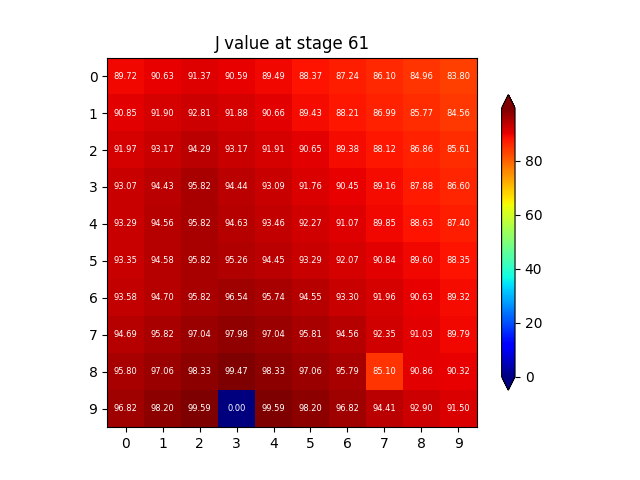
\includegraphics[angle=0,width=0.6\textwidth]{hw2/logs/t=3_N=-1/J-heatmap-61.png}
\caption{Heat-map of $J_i$ till absolute difference convergence for \textbf{Terminal State (3,0)}}
\end{subfigure}

\begin{subfigure}
\centering
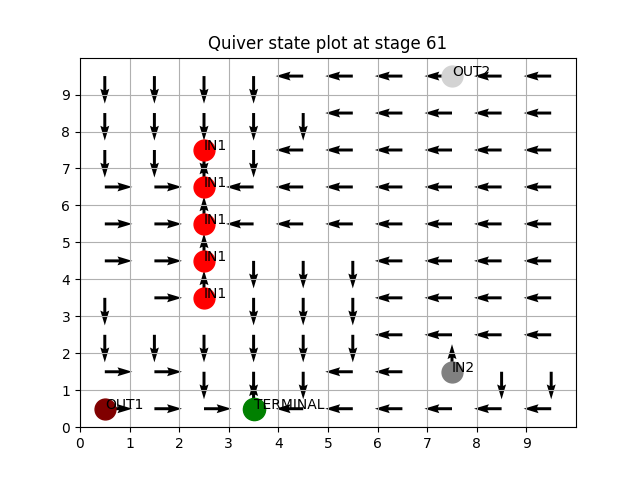
\includegraphics[angle=0,width=0.6\textwidth]{hw2/logs/t=3_N=-1/quiver-61.png}
\caption{Quiver plot of $\pi$  till absolute difference convergence for \textbf{Terminal State (3,0)}}
\end{subfigure}
\end{figure}

\section {Question 2: Taxi Driver Problem}

Dynamic Programming via the compact Bellman operators was used to solve this problem.

We implement $T(J)$ by the following vectorised code:
\begin{lstlisting}[numbers = none]
np.amax(np.sum(r*P+P*np.expand_dims(J.T,2),axis=1),axis=1)
\end{lstlisting}

We get past the fact that at \textit{town B } you cannot take action 3 (or our action 2) , by settting the rewards for action 2 (for B) as zero. Also note that since python indexing begins at zero, so do our numbering of states, stages and actions.

Where, $r$ is the reward matrix of shape (states, states, actions);
$P$ is the probability matrix of shape (states, states, actions);
$J$ is the set of states.

We do not assume the policy to be stationary (stage independent), however, this turns out to be the case in the optimal policy.

The results may be reproduced by running:
\begin{lstlisting}[numbers = none]
python3 q2.py --iter_type value
\end{lstlisting}

Here, iteration type is one of "value", "policy", "mpi", "gauss".

\subsection{Part 1}

Solving via policy iteration, $\beta$ varying from 0 to 0.95.

\begin{lstlisting}[numbers = none]
BETA 0.0
Policy Iteration: Starting with initial policy [0 0 0]
Final optimal policy
{'state 0': 'action 0', 'state 1': 'action 0', 'state 2': 'action 0'}
Final optimal cost
[ 8.   16.    7.]


 ------------ 


BETA 0.05
Policy Iteration: Starting with initial policy [0 0 0]
Final optimal policy
{'state 0': 'action 0', 'state 1': 'action 0', 'state 2': 'action 0'}
Final optimal cost
[ 8.511527  16.400260   7.498869]


 ------------ 


BETA 0.1
Policy Iteration: Starting with initial policy [0 0 0]
Final optimal policy
{'state 0': 'action 0', 'state 1': 'action 0', 'state 2': 'action 0'}
Final optimal cost
[ 9.076506  16.856369   8.05866 ]


 ------------ 


BETA 0.15
Policy Iteration: Starting with initial policy [0 0 0]
Final optimal policy
{'state 0': 'action 0', 'state 1': 'action 0', 'state 2': 'action 1'}
Final optimal cost
[ 9.704506  17.385855   8.665495 ]


 ------------ 


BETA 0.2
Policy Iteration: Starting with initial policy [0 0 0]
Final optimal policy
{'state 0': 'action 0', 'state 1': 'action 0', 'state 2': 'action 1'}
Final optimal cost
[ 10.646457  18.582842   9.358115]


 ------------ 


BETA 0.25
Policy Iteration: Starting with initial policy [0 0 0]
Final optimal policy
{'state 0': 'action 0', 'state 1': 'action 0', 'state 2': 'action 1'}
Final optimal cost
[ 11.200000  19.76897117   10.128867]


 ------------ 


BETA 0.3
Policy Iteration: Starting with initial policy [0 0 0]
Final optimal policy
{'state 0': 'action 0', 'state 1': 'action 0', 'state 2': 'action 1'}
Final optimal cost
[ 12.102002  20.78557   11.020489  ]


 ------------ 


BETA 0.35
Policy Iteration: Starting with initial policy [0 0 0]
Final optimal policy
{'state 0': 'action 0', 'state 1': 'action 0', 'state 2': 'action 1'}
Final optimal cost
[ 13.136027  22.258473  12.048413]


 ------------ 


BETA 0.4
Policy Iteration: Starting with initial policy [0 0 0]
Final optimal policy
{'state 0': 'action 0', 'state 1': 'action 0', 'state 2': 'action 1'}
Final optimal cost
[ 13.268198  22.254607  12.042691]


 ------------ 


BETA 0.45
Policy Iteration: Starting with initial policy [0 0 0]
Final optimal policy
{'state 0': 'action 0', 'state 1': 'action 0', 'state 2': 'action 1'}
Final optimal cost
[ 15.78263383  26.014349  14.630118]


 ------------ 


BETA 0.5
Policy Iteration: Starting with initial policy [0 0 0]
Final optimal policy
{'state 0': 'action 0', 'state 1': 'action 1', 'state 2': 'action 1'}
Final optimal cost
[ 17.054971  28.453838  16.674914]


 ------------ 


BETA 0.55
Policy Iteration: Starting with initial policy [0 0 0]
Final optimal policy
{'state 0': 'action 0', 'state 1': 'action 1', 'state 2': 'action 1'}
Final optimal cost
[ 19.604929  31.423986  19.867081]


 ------------ 


BETA 0.6
Policy Iteration: Starting with initial policy [0 0 0]
Final optimal policy
{'state 0': 'action 0', 'state 1': 'action 1', 'state 2': 'action 1'}
Final optimal cost
[ 22.812414  35.143268  23.208965]


 ------------ 


BETA 0.65
Policy Iteration: Starting with initial policy [0 0 0]
Final optimal policy
{'state 0': 'action 1', 'state 1': 'action 1', 'state 2': 'action 1'}
Final optimal cost
[ 26.960790  39.858200  27.533954]


 ------------ 


BETA 0.7
Policy Iteration: Starting with initial policy [0 0 0]
Final optimal policy
{'state 0': 'action 1', 'state 1': 'action 1', 'state 2': 'action 1'}
Final optimal cost
[ 32.523392  46.265610  34.257728]


 ------------ 


BETA 0.75
Policy Iteration: Starting with initial policy [0 0 0]
Final optimal policy
{'state 0': 'action 1', 'state 1': 'action 1', 'state 2': 'action 1'}
Final optimal cost
[ 41.354247  55.128817  43.257070]


 ------------ 


BETA 0.8
Policy Iteration: Starting with initial policy [0 0 0]
Final optimal policy
{'state 0': 'action 1', 'state 1': 'action 1', 'state 2': 'action 1'}
Final optimal cost
[ 55.16560   68.235668  56.248407]


 ------------ 


BETA 0.85
Policy Iteration: Starting with initial policy [0 0 0]
Final optimal policy
{'state 0': 'action 1', 'state 1': 'action 1', 'state 2': 'action 1'}
Final optimal cost
[ 77.246512  90.713441    78.243455]


 ------------ 


BETA 0.9
Policy Iteration: Starting with initial policy [0 0 0]
Final optimal policy
{'state 0': 'action 1', 'state 1': 'action 1', 'state 2': 'action 1'}
Final optimal cost
[ 121.653471  135.316770   122.836810 ]


 ------------ 


BETA 0.95
Policy Iteration: Starting with initial policy [0 0 0]
Final optimal policy
{'state 0': 'action 1', 'state 1': 'action 1', 'state 2': 'action 1'}
Final optimal cost
[ 255.022908  268.764619  256.202849]

\end{lstlisting}

Clearly, the optimal policy is stationary and equal to:
\begin{lstlisting}[numbers = none]
Optimal policy is {'state 0': 'action 1', 'state 1': 'action 1', 'state 2': 'action 2'}
\end{lstlisting}

ie, ...,

\begin{itemize}
\item For towns A, B, C:  Go to the nearest taxi stand and wait in line.
\end{itemize}

Some comments on the rewards and policy:
\begin{itemize}
\item The rewards are bounded - saturate to a fixed point - with stage. This is expected since there is a concept of termination in this problem, due to the presence of a discount factor.
\item More the discount factor, faster you terminate, and hence lower the reward. The limit that $\beta$ tends to 1, we get infinite reward.
\item We do not end up with action 3 for \textit{town B} - a sanity check.
\end{itemize}

\subsection{Part 2}

We repeat with modified policy iteration with $m_k = 5 $, starting policy as cruise (corresponds to [0,0,0])

\begin{lstlisting}
BETA 0.9

Modified Policy Iteration: Starting with initial policy [0 0 0]
Final optimal policy
{'state 0': 'action 1', 'state 1': 'action 1', 'state 2': 'action 1'}
Final MPI cost
[ 121.618512  135.206776   122.297678 ]
\end{lstlisting}

We notice a deviation between the "MPI" cost, and the actual $J_\pi$ associated with the optimal policy, this is due to the approximation made by MPI.

However, we still converge to the same policy.

Also, the approximation improves as $m_k$ tends to infinity. In specific for $m_k$ =10:

\begin{lstlisting}
BETA 0.9

Modified Policy Iteration: Starting with initial policy [0 0 0]
Final optimal policy
{'state 0': 'action 1', 'state 1': 'action 1', 'state 2': 'action 2'}
Final MPI cost
[ 121.618533  135.816778   122.297891 ]
\end{lstlisting}


\subsection{Code Snippet for MPI} 

\begin{lstlisting}
def modified_policy_iter(actions, m_k=5, alpha=0.9, verbose=False):
    # Helper vars
    actions_array = []
    J_array = []
    counter = 0

    i = list(range(3))

    while True:
        # Policy evaluation
        actions_array.append(actions)
        # div = np.eye(3) - alpha *P[i, :, actions[i]]
        # div = np.linalg.inv(div)

        # J = np.sum(r[i, :, actions[i]] *
        #             P[i, :, actions[i]], axis=1)
        # J = np.dot(div, J)

        # Perform value iteration m_k times
        J = np.zeros(3)
        for i in range(m_k):
            J = T(J, alpha=alpha)

        J_array.append(J)

        if verbose:
            print(f"J value {J}")

        # Policy improvement
        actions_new = read_optimal_policy(J)

        if np.max(np.abs(actions_new - actions)) == 0:
            if verbose:
                print(f"Counter value {counter}  \n\n")
            actions = read_optimal_policy(J, verbose=verbose)
            break
        else:
            actions = actions_new
            counter += 1

    return J_array, actions_array
\end{lstlisting}

\subsection{Part 3: Value Iteration and Gauss Seidel}

Here, we use gauss seidel as an approximation or variant to value iteration, where we randomly update a single state. \\

With Gauss Seidel method and $\beta = 0.9$: ( we enlist the iterations needed to converge within $\epsilon = 1e-6$ too)

\begin{lstlisting}
BETA 0.9

Gauss Seidel Iteration: 

Starting with end stage costs as [ 0.  0.  0.]
Iterations needed : 
411
Optimal policy is :
{'state 0': 'action 1', 'state 1': 'action 1', 'state 2': 'action 2'}
Cost is : 
[121.653471  135.316770   122.836810]
\end{lstlisting}

With Value Iteration method and $\beta = 0.9$: (we run till convergence of $1e-4$)

\begin{lstlisting}
BETA 0.9

 Value Iteration: Starting with end stage costs as [ 0 0 0]
Optimal policy is 
{'state 0': 'action 1', 'state 1': 'action 1', 'state 2': 'action 1'}
[121.653471  135.316770   122.836810]
\end{lstlisting}

\subsection {Code Blocks (Gauss Seidel)}
\begin{lstlisting}
def gauss_siedel(J, alpha=0.9, verbose=True, epi=1e-6):
    actions_array = []
    J_array = []

    count = 0

    while True:

        # Randomly update a state
        r = np.random.randint(3)
        up = T(J, alpha=alpha)[r]
        diff = J[r] - up
        J[r] = up

        if verbose:
            print(f"Count {count}")
            print(f"Values of J {J} at stage {count}")
            print(f"Optimal policy is at stage {count} is")
            actions_array.append(
                read_optimal_policy(
                    J, verbose=verbose, alpha=alpha))
        else:
            actions_array.append(
                read_optimal_policy(
                    J, verbose=verbose, alpha=alpha))

        if np.abs(diff) < epi:
            break

        else:
            J_array.append(J)
            count += 1

    print(f"Iterations needed : \n{count}")
    print("Optimal policy is :")
    read_optimal_policy(J, alpha=alpha, verbose=True)
    print(f"Cost is : \n{J}")

    return J_array, actions_array
\end{lstlisting}
\bigskip

% References
\section{References}
\begin{itemize}
\item Classroom lectures.
\item Bertsekas:\textit{ Dynamic Programming and Optimal Control, Vol 2, 3rd ed.}
\item Numpy, Matplotlib Dev Documentation.
\end{itemize}


\end{document}